\subsection{Problema a resolver}

El siguiente ejercicio se da en el contexto de un museo donde se requiere, por cuestiones de seguridad, colocar sensores de forma tal que todo el piso del museo esté cubierto por los laser que emiten, existen dos tipos de sensores, lo direccionales (que emiten señales horizontales o verticales) y los bidireccionales (que emiten señales hacia ambos lados) y su valor es \$4000 y \$6000 respectivamente. Se pide también que un sensor no este apuntando hacia otro por que esto podria provocar que algún sensor deje de funcionar y no es lo deseado, ademas se pide que en ciertos lugares, definidos como "importantes", haya dos laser pasando simulateamente. El objetivo entonces es encontrar la forma de colocar estos sensores de forma tal que el suelo quede completamente cubierto y que los lugares importantes queden con ambos laser pasando por el y ademas que el costo total de los sensores sea minimo, tambien hay que tener en cuenta que en el museo puede haber paredes que interfieran en los laser de los sensores.

Un ejemplo de este problema es el que está provisto por la catedra


\begin{figure}[H]
	\begin{center}
		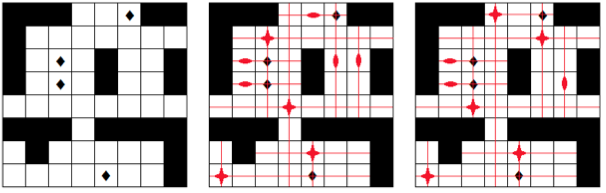
\includegraphics[width=320pt]{../imgs/ej3_ejemploCatedra.png}
	\end{center}
\caption{Un ejemplo y dos soluciones distintas.}
\end{figure}

En el ejemplo de la Figura 1 el museo se ve representado por una cuadricula donde donde los cuadrados blancos representan el suelo, los cuadrados negros representan las paredes y los cuadrados que tienen un rombo dentro representan los lugares importantes, a continuacion de la imagen se muetran dos posibles soluciones al problema, en las cuales las cruces rojas representan los sensores bidireccionales, y las lineas rojas gruesas representan los sensores horizontales y verticales, desde estos sensores se extienden lineas rojas que representan el area que cubren estos sensores.

En el primer caso el costo total es de \$44000 y la segunda solucion tiene un costo de \$42000

\subsection{Resolución coloquial}

\subsection{Demostración de correctitud}

\subsection{Complejidad del algoritmo}

\subsection{Código fuente}

\subsection{Instancias posibles}

\subsection{Testing}
